\documentclass[pdf]{beamer}
\usepackage[latin1]{inputenc}
\usepackage{multirow}
\usetheme{Goettingen} %Warsaw
\usecolortheme{seagull}

%\usepackage{movie15}

\begin{document}

\title[Introduction to Sequencing]{Introduction to Sequencing}
\subtitle{BCB 504: Applied Bioinformatics\\}
\author[Matt Settles]{Matt Settles}
\institute{University of Idaho\\ Bioinformatics and Computational Biology Program}
\date{\today}


%% Title page
\begin{frame}[plain]
  \titlepage
\end{frame}


%% Outline
\begin{frame}[plain] 
  \frametitle{Outline}
  \tableofcontents
\end{frame}

\section{History}
\begin{frame}
  \frametitle{Evolution of DNA Sequencing}
  {\footnotesize Oct - 2012: \$0.07 per Megabase, \$6,618 per Human Sized Genome (30x coverage)}
  \begin{center}
  \begin{figure}
    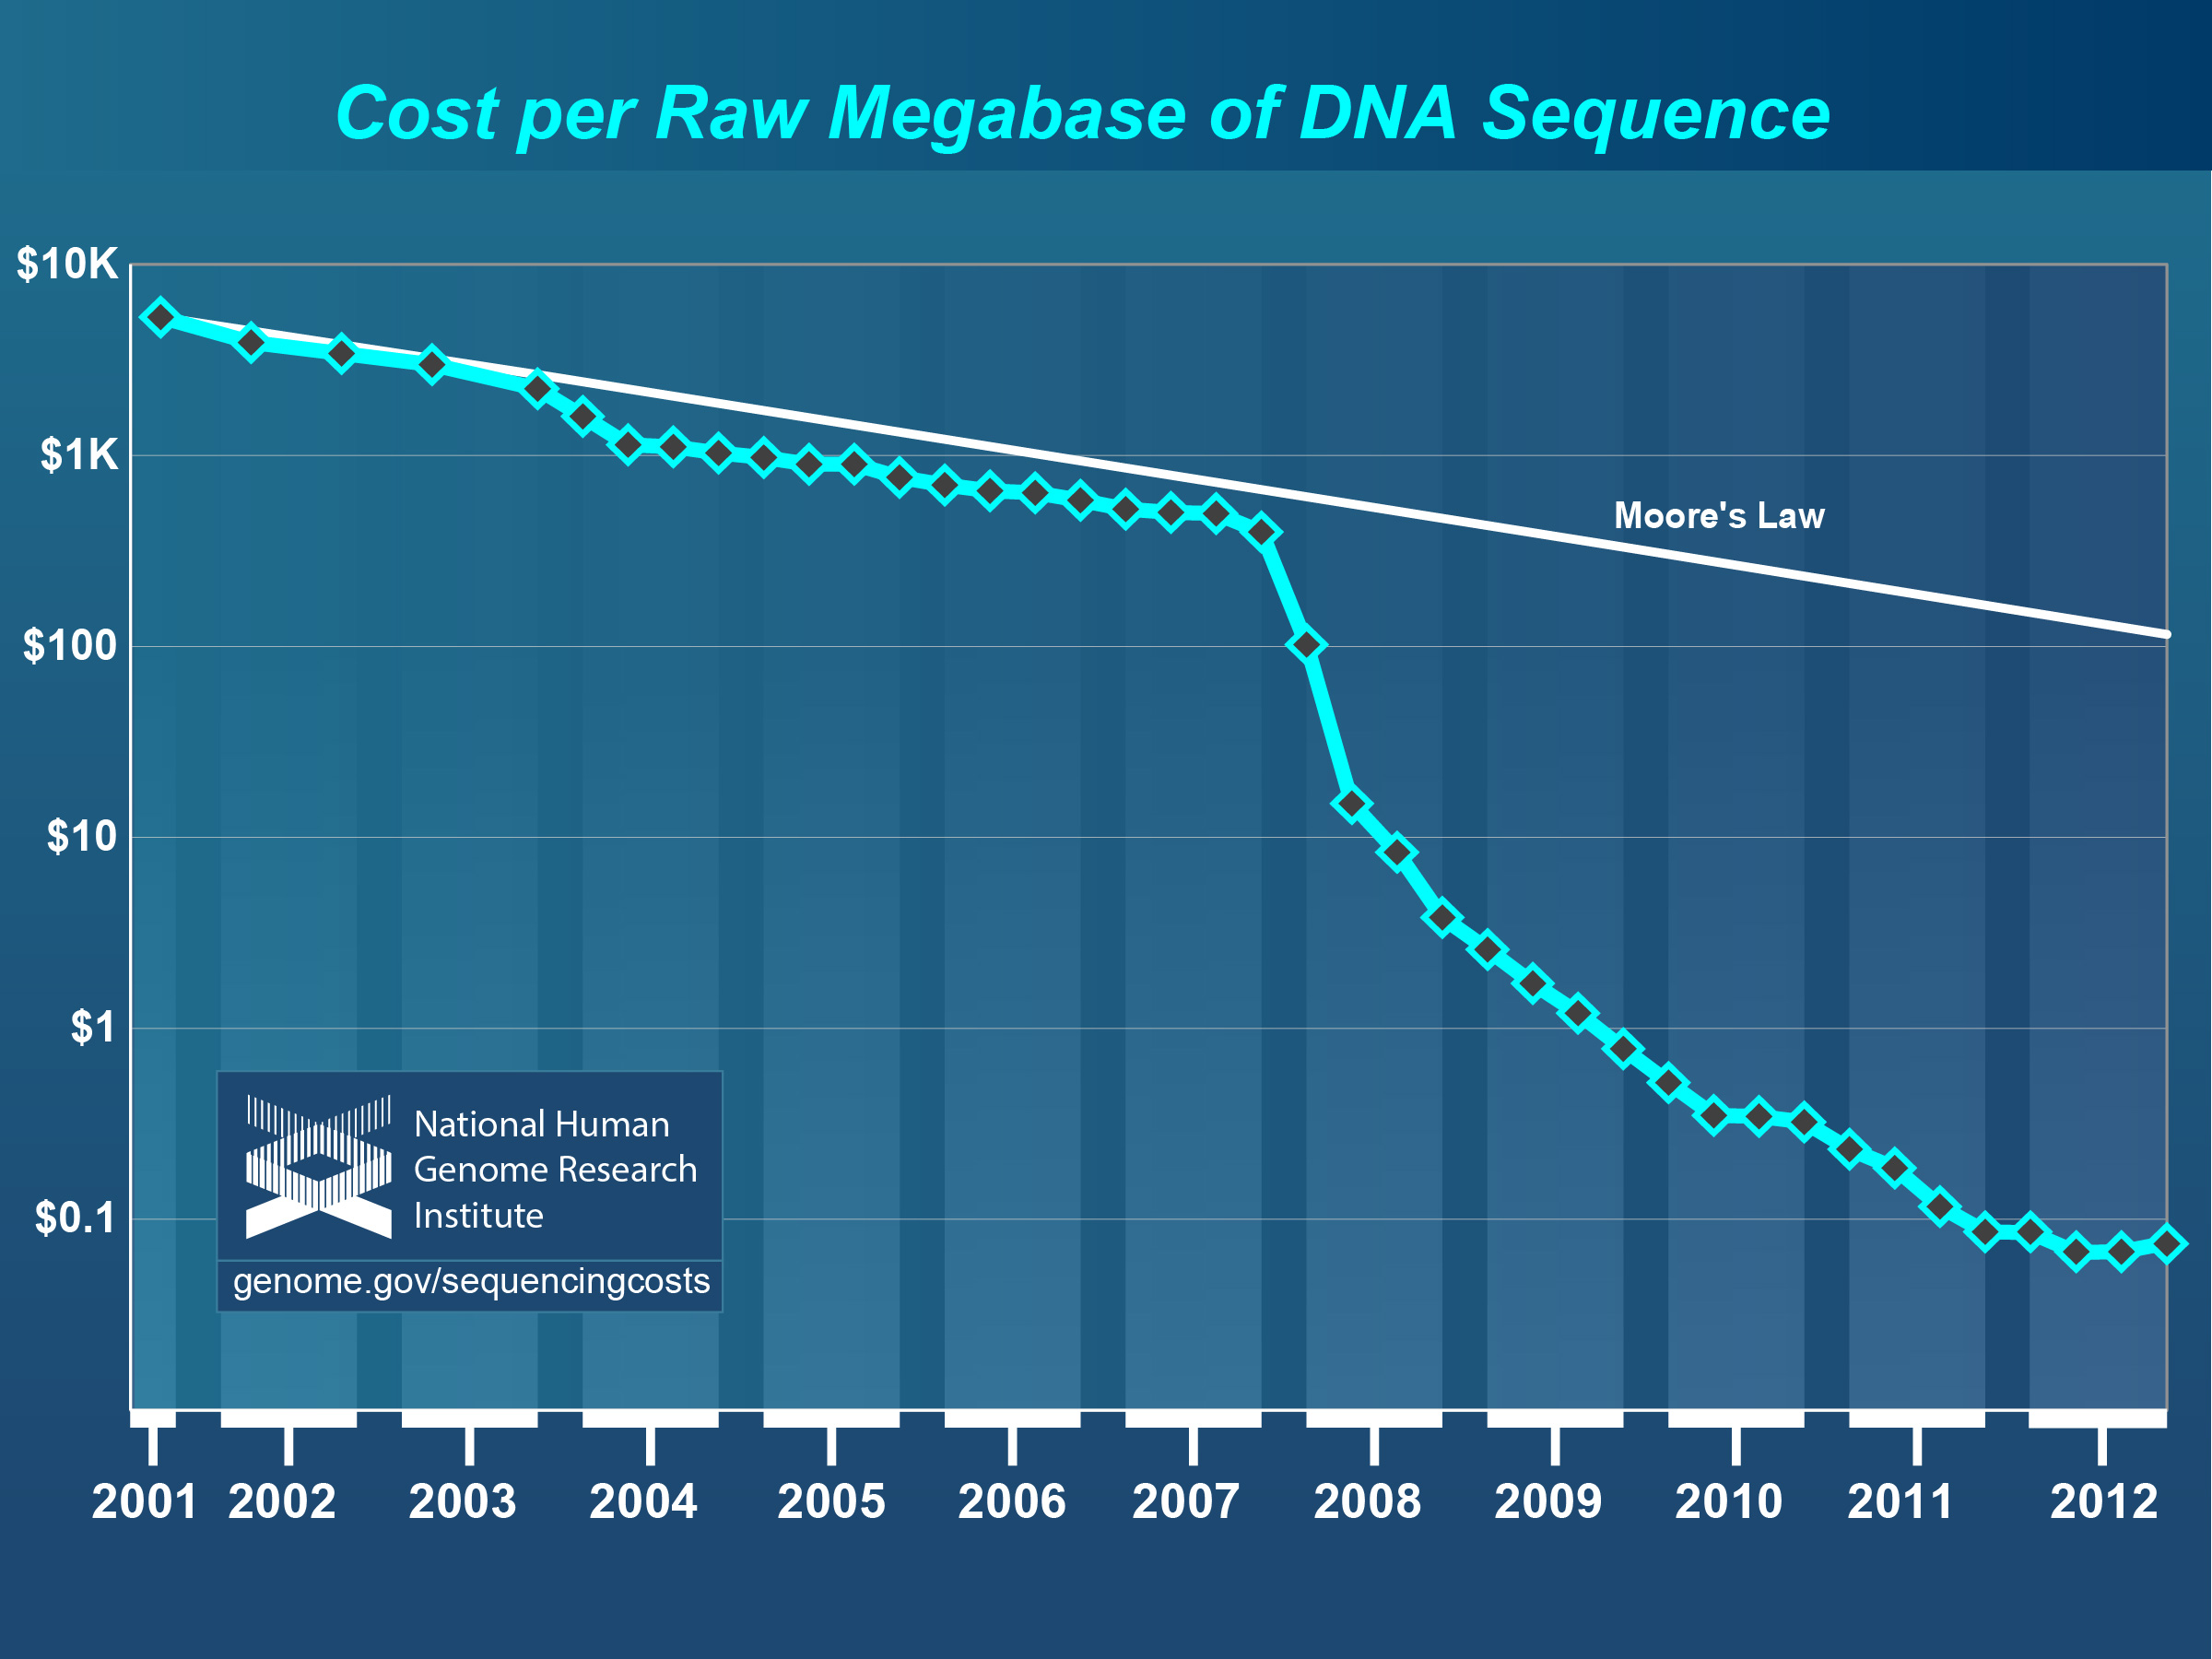
\includegraphics[scale=0.4]{cost_per_megabase.jpg}
  \end{figure}
  \end{center}
\end{frame}

\section{Roche 454 Pyrosequencing}

\begin{frame}
  \frametitle{Roche 454}
  The first massively parallel method to become commercially available was developed by 454 Life Sciences in 2005 (acquired by Roche in 2007) and is based on the pyrosequencing technique. Similar to the Sanger method, sequencing is carried out using primed synthesis by DNA polymerase. However in the 454 pyrosequencing method, the DNA fragments are presented with each of the four dNTPs sequencially and without a dye-terminator, as is done with Sanger sequencing, allowing for multiple incorportation in the same flow. The amount of the incorporation is monitored by luminometric detection of the pyrophosphate released (hence the name "pyrosequencing").
\end{frame}

\begin{frame}
  \frametitle{Roche 454 platforms}
  Roche 454 has 2 platforms the GS Junior System (a "benchtop" system) and the GS FLX+ System (what we have on campus).
  \begin{center}
    \begin{figure}
    \includegraphics[scale=0.4]{Roche_specs.png}
  \end{figure}
  \end{center}
\end{frame}

\begin{frame}
  \frametitle{Roche 454 Workflow Video}
  \begin{center}
  \href{http://www.youtube.com/watch?feature=player_detailpage&v=bFNjxKHP8Jc}{454 Video}
  \end{center}  
\end{frame}

\begin{frame}
  \frametitle{Roche 454 Workflow}
  \begin{itemize}
  \item Library Construction
  \item QA - Library Quantification (Titration)
  \item emulsion PCR (emPCR)
  \item Picotiter Plate Loading
  \item Sequencing
  \item Image extraction
  \item Flowgram extraction
  \end{itemize}
\end{frame}


\begin{frame}
  \frametitle{Roche 454 Flowgrams}
  \begin{center}
    \begin{figure}
    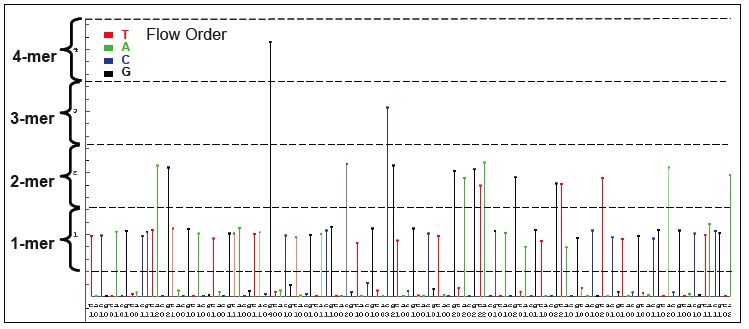
\includegraphics[scale=0.35]{Flowgram.jpg}
  \end{figure}
  \end{center}
\end{frame}

\begin{frame}
  \frametitle{454 Read Naming Convections}
Roche 454 raw data are stored in SFF files (standard flowgram format), but fasta and qual (or fastq) files can be extracted from them\\
  $>$EBO6PME01EGNVK
  \begin{description}
  \item[Timestamp] EB06PM
  \item[Randomized ] E
  \item[Plate Region] 01
  \item[X,Y coord] EGNVK
  \end{description}
  The timestamp, hash character and X,Y location use a base-36 encoding (where values 0-25 are the letters 'A'-'Z' and the values 26-35 are the digits '0'-'9'). An accession thus consists only of letters and digits, and is case-insensitive. 
\end{frame}
   

\section{Illumina Solexa}

\begin{frame}
  \frametitle{Illumina Solexa}
  The second next-generation sequencing technology to be released (in 2006) was Illumina Solexa sequencing. A key difference between Roche 454 and Illumina sequencing was the suse of chain-terminating nucleotides. The fluorescent label on the terminating base can be removed to leave an unblocked 3' terminus, mating the chain termination a reversible process. The method thus sequences at a time, rather than multiple bases (in a homopolymer run) as does Roche 454.
\end{frame}

\begin{frame}
  \frametitle{Illumina Platforms}
  Illumina currently has 2 platforms, the MiSeq benchtop version (what we have on campus) and the HiSeq (with 4 variations).
    \begin{center}
    \begin{figure}
    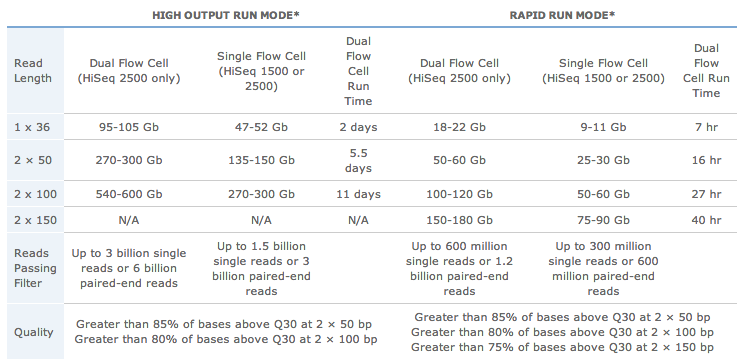
\includegraphics[scale=0.38]{Illumina_specs.png}
  \end{figure}
  \end{center}
\end{frame}

\begin{frame}
  \frametitle{Illumina Workflow Video}
  \begin{center}
  \href{http://www.youtube.com/watch?NR=1&feature=endscreen&v=l99aKKHcxC4}{Illumina Video}
  \end{center}
\end{frame} 

  
\begin{frame}
  \frametitle{Illumina Workflow}
  \begin{itemize}
  \item Library Construction
  \item Cluster Generation
  \item Sequencing
  \item image extraction
  \end{itemize}
\end{frame}
  
\begin{frame}
  \frametitle{Illumina Read Naming Conventions}
  \begin{small}
  @EAS139:136:FC706VJ:2:2104:15343:197393 1:Y:18:ATCACG\\
  \end{small}  
  \begin{description}
  \item[EAS139]	the unique instrument name
  \item[136]	the run id
  \item[FC706VJ]	the flowcell id
  \item[2]	flowcell lane
  \item[2104]	tile number within the flowcell lane
  \item[15343]	'x'-coordinate of the cluster within the tile
  \item[197393]	'y'-coordinate of the cluster within the tile
  \item[1]	the member of a pair, 1 or 2 (paired-end or mate-pair reads only)
  \item[Y]	Y if the read fails filter (read is bad), N otherwise
  \item[18]	0 when none of the control bits are on, otherwise it is an even     number
  \item[ATCACG]	index sequence
  \end{description}
\end{frame}

\section{Sequence Data}
\begin{frame}
  \frametitle{fasta,qual and fastq files}
  \begin{itemize}
  \item fasta files\\%
  $>$sequence1\\
  ACCCATGATTTGCGA
  \item qual files\\%
  $>$sequence1\\
  40 40 39 39 40 39 40 40 40 40 20 20 36 39 39
  \item fastq files\\%
  $@$sequence1\\
  ACCCATGATTTGCGA\\
  $+$\\
  IIHHIHIIII55EHH
  \end{itemize}
\end{frame}

\begin{frame}
  \frametitle{phred scores}
$Q = -10log_{10}P$
\begin{center}
\begin{tabular}{|l|l|l|}
\hline
Phred & Probability &	Base call \\
Quality Score	& of incorrect  & accuracy \\
 & base call & \\
\hline
10	&	1 in 10	&	$90\%$\\
20	&	1 in 100 &	$99\%$\\
30	&	1 in 1000	&	$99.9\%$\\
40	&	1 in 10000	&	$99.99\%$\\
\hline
\end{tabular}
\end{center}
\end{frame}
% fasta
% qual
% fastq
%% quality scores
\begin{frame}
  \frametitle{phred score conversion}
$Q_{sanger} = -10log_{10}P$ - based on probability (aka phred)
\\

$Q_{solexa} = -10log_{10}\frac{P}{1-P}$ - based on odds
\begin{center}
\begin{tabular}{ l l l }
S - Sanger        &Phred+33,  &raw reads typically (0, 40) \\
X - Solexa        &Solexa+64, &raw reads typically (-5, 40) \\
I - Illumina 1.3+ &Phred+64,  &raw reads typically (0, 40) \\
J - Illumina 1.5+ &Phred+64,  &raw reads typically (3, 40) \\
L - Illumina 1.8+ &Phred+33,  &raw reads typically (0, 41) \\
\end{tabular}
\end{center}
\end{frame} 


\section{Library Preparation}
\begin{frame}
 \frametitle{Library Preparation types}
 \begin{itemize}
 \item Shotgun - randomly fragmented DNA (100bp - 1kb) 
 \item RNA - Random nanomers or 3' bias (stranded or unstranded)
 \item Amplicons
 \item Paired end / Mate pair
 \end{itemize}
\end{frame} 

\section{Other sequencing technologies}
\begin{frame}
  \frametitle{Ion Torrent Workflow Video}
Ion Torrent, first available in 2011, generates up to 400bp reads (reported) and up to 2Gb per run. Cheap fast runs. Ion Proton system available soon(?). 200-bp fragments and up to 10Gb per run. Generates flowgrams and SFF files similar to Roche 454 data.
  \begin{center}
  \href{http://www.youtube.com/watch?v=jbVbddI2Hpg}{Ion Torrent Video}
  \end{center}
\end{frame} 


\begin{frame}
Pacific Biosystems is so far the most sucessful third generation DNA sequencing system. Key differences are that its a single molecule, real time technology and capable of producing sequences of multi kilobases.
  \frametitle{Pacific Biosciences Workflow Video}
  \begin{center}
  \href{http://www.youtube.com/watch?v=NHCJ8PtYCFc&feature=endscreen&NR=1}{Pacific Biosciences Video}
  \end{center}
  \begin{center}
    \begin{figure}
    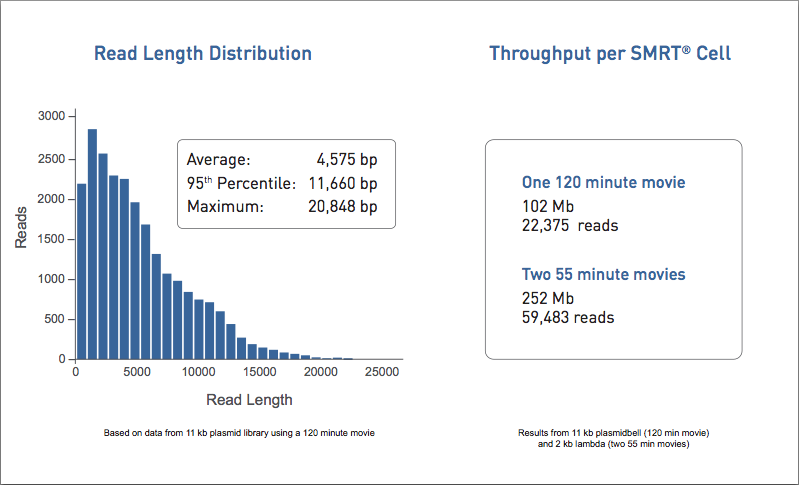
\includegraphics[scale=0.30]{PacBio-specs.png}
  \end{figure}
  \end{center}

\end{frame} 


\end{document}

